\section{Simulation scenarios}

The simulations were carried out under four different agents-obstacles
configurations:

\begin{enumerate}
  \item Two agents avoid one obstacle on their way to their
    steady-state configurations, without colliding with each other and without
    being separated by the obstacle (we demand that their distance is always
    smaller than the obstacle's diameter for the aim of cooperation).
  \item Two agents pass through the space between two obstacles
    on their way to their steady-state configurations $-$ again, the maximum
    allowed distance between the two agents is smaller than the diameter
    of the obstacle with the smallest radius.
  \item Three agents avoid one obstacle on their way to their
    steady-state configurations, without colliding with each other and without
    being separated by the obstacle. In this case, two agents are
    (independently) neighbours of the third, that is, the third agent should
    maintain connectivity and avoid collision with both of the other two,
    but the latter will only have to avoid colliding with each other.
  \item Three agents pass through the space between two obstacles
    on their way to their steady-state configurations. The conditions of this
    scenario assume those of points 2 and 3.
\end{enumerate}

The four configurations are depicted in figures \eqref{fig:test_case_2_1},
\eqref{fig:test_case_2_2}, \eqref{fig:test_case_3_1} and
\eqref{fig:test_case_3_2}. Agent 1 is depicted in blue, agent 2 in
red and agent 3 in yellow. The obstacles are depicted in black. A faint line
connects neighbouring agents; it is coloured in green. Mark X
denotes the desired position of an agent and its colour signifies the agent
to be stabilized in that position.


\noindent\makebox[\linewidth][c]{%
\begin{minipage}{\linewidth}
  \begin{minipage}{0.45\linewidth}
    \begin{figure}[H]
      \scalebox{0.7}{% This file was created by matlab2tikz.
%
%The latest updates can be retrieved from
%  http://www.mathworks.com/matlabcentral/fileexchange/22022-matlab2tikz-matlab2tikz
%where you can also make suggestions and rate matlab2tikz.
%
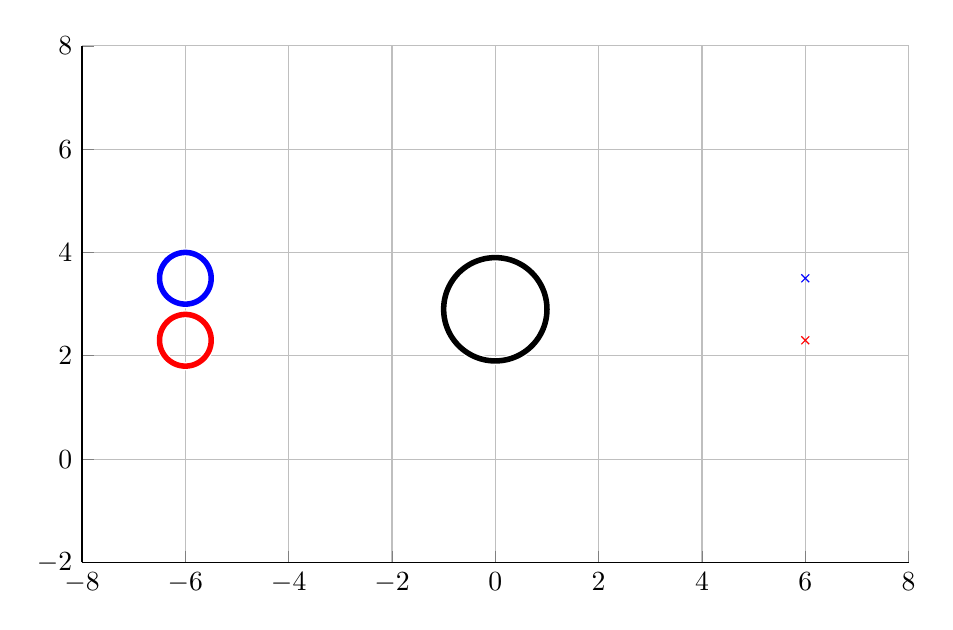
\begin{tikzpicture}

\begin{axis}[%
width=4.133in,
height=2.583in,
at={(0.693in,0.778in)},
scale only axis,
unbounded coords=jump,
xmin=-8,
xmax=8,
xmajorgrids,
ymin=-2,
ymax=8,
ymajorgrids,
axis background/.style={fill=white},
axis x line*=bottom,
axis y line*=left
]
\addplot [color=blue,only marks,mark=x,mark options={solid},forget plot]
  table[row sep=crcr]{%
6	3.5\\
};
\addplot [color=red,only marks,mark=x,mark options={solid},forget plot]
  table[row sep=crcr]{%
6	2.3\\
};
\addplot [color=white,solid,line width=3.0pt,forget plot]
  table[row sep=crcr]{%
-5.5	3.5\\
-5.50030458649045	3.51744974835125\\
-5.50121797487009	3.53487823687206\\
-5.50273905231586	3.55226423163383\\
-5.50486596562921	3.56958655048003\\
-5.5075961234939	3.58682408883347\\
-5.5109261996331	3.60395584540888\\
-5.514852136862	3.62096094779983\\
-5.51936915203084	3.6378186779085\\
-5.52447174185242	3.65450849718747\\
-5.53015368960705	3.67101007166283\\
-5.53640807271661	3.68730329670796\\
-5.5432272711787	3.7033683215379\\
-5.55060297685042	3.71918557339454\\
-5.55852620357054	3.73473578139295\\
-5.56698729810778	3.75\\
-5.57597595192179	3.7649596321166\\
-5.58548121372248	3.77959645173537\\
-5.59549150281253	3.79389262614624\\
-5.60599462319664	3.80783073766283\\
-5.61697777844051	3.82139380484327\\
-5.6284275872613	3.83456530317943\\
-5.64033009983067	3.8473291852295\\
-5.6526708147705	3.85966990016933\\
-5.66543469682057	3.8715724127387\\
-5.67860619515673	3.88302222155949\\
-5.69216926233717	3.89400537680336\\
-5.70610737385376	3.90450849718747\\
-5.72040354826463	3.91451878627752\\
-5.7350403678834	3.92402404807821\\
-5.75	3.93301270189222\\
-5.76526421860705	3.94147379642946\\
-5.78081442660546	3.94939702314958\\
-5.7966316784621	3.9567727288213\\
-5.81269670329204	3.96359192728339\\
-5.82898992833717	3.96984631039295\\
-5.84549150281253	3.97552825814758\\
-5.8621813220915	3.98063084796916\\
-5.87903905220017	3.985147863138\\
-5.89604415459112	3.9890738003669\\
-5.91317591116653	3.9924038765061\\
-5.93041344951997	3.99513403437079\\
-5.94773576836617	3.99726094768414\\
-5.96512176312794	3.99878202512991\\
-5.98255025164875	3.99969541350955\\
-6	4\\
-6.01744974835125	3.99969541350955\\
-6.03487823687206	3.99878202512991\\
-6.05226423163383	3.99726094768414\\
-6.06958655048003	3.99513403437079\\
-6.08682408883347	3.9924038765061\\
-6.10395584540888	3.9890738003669\\
-6.12096094779983	3.985147863138\\
-6.1378186779085	3.98063084796916\\
-6.15450849718747	3.97552825814758\\
-6.17101007166283	3.96984631039295\\
-6.18730329670796	3.96359192728339\\
-6.2033683215379	3.9567727288213\\
-6.21918557339454	3.94939702314958\\
-6.23473578139295	3.94147379642946\\
-6.25	3.93301270189222\\
-6.2649596321166	3.92402404807821\\
-6.27959645173537	3.91451878627752\\
-6.29389262614624	3.90450849718747\\
-6.30783073766283	3.89400537680336\\
-6.32139380484327	3.88302222155949\\
-6.33456530317943	3.8715724127387\\
-6.3473291852295	3.85966990016933\\
-6.35966990016933	3.8473291852295\\
-6.3715724127387	3.83456530317943\\
-6.38302222155949	3.82139380484327\\
-6.39400537680336	3.80783073766283\\
-6.40450849718747	3.79389262614624\\
-6.41451878627752	3.77959645173537\\
-6.42402404807821	3.7649596321166\\
-6.43301270189222	3.75\\
-6.44147379642946	3.73473578139295\\
-6.44939702314958	3.71918557339454\\
-6.4567727288213	3.7033683215379\\
-6.46359192728339	3.68730329670796\\
-6.46984631039295	3.67101007166283\\
-6.47552825814758	3.65450849718747\\
-6.48063084796916	3.6378186779085\\
-6.485147863138	3.62096094779983\\
-6.4890738003669	3.60395584540888\\
-6.4924038765061	3.58682408883347\\
-6.49513403437079	3.56958655048003\\
-6.49726094768414	3.55226423163383\\
-6.49878202512991	3.53487823687206\\
-6.49969541350955	3.51744974835125\\
-6.5	3.5\\
-6.49969541350955	3.48255025164875\\
-6.49878202512991	3.46512176312794\\
-6.49726094768414	3.44773576836617\\
-6.49513403437079	3.43041344951997\\
-6.4924038765061	3.41317591116653\\
-6.4890738003669	3.39604415459112\\
-6.485147863138	3.37903905220017\\
-6.48063084796916	3.3621813220915\\
-6.47552825814758	3.34549150281253\\
-6.46984631039295	3.32898992833717\\
-6.46359192728339	3.31269670329204\\
-6.4567727288213	3.2966316784621\\
-6.44939702314958	3.28081442660546\\
-6.44147379642946	3.26526421860705\\
-6.43301270189222	3.25\\
-6.42402404807821	3.2350403678834\\
-6.41451878627752	3.22040354826463\\
-6.40450849718747	3.20610737385376\\
-6.39400537680336	3.19216926233717\\
-6.38302222155949	3.17860619515673\\
-6.3715724127387	3.16543469682057\\
-6.35966990016933	3.1526708147705\\
-6.3473291852295	3.14033009983067\\
-6.33456530317943	3.1284275872613\\
-6.32139380484327	3.11697777844051\\
-6.30783073766283	3.10599462319664\\
-6.29389262614624	3.09549150281253\\
-6.27959645173537	3.08548121372248\\
-6.2649596321166	3.07597595192179\\
-6.25	3.06698729810778\\
-6.23473578139295	3.05852620357054\\
-6.21918557339454	3.05060297685042\\
-6.2033683215379	3.0432272711787\\
-6.18730329670796	3.03640807271661\\
-6.17101007166283	3.03015368960705\\
-6.15450849718747	3.02447174185242\\
-6.1378186779085	3.01936915203084\\
-6.12096094779983	3.014852136862\\
-6.10395584540888	3.0109261996331\\
-6.08682408883347	3.0075961234939\\
-6.06958655048003	3.00486596562921\\
-6.05226423163383	3.00273905231586\\
-6.03487823687206	3.00121797487009\\
-6.01744974835125	3.00030458649045\\
-6	3\\
-5.98255025164875	3.00030458649045\\
-5.96512176312794	3.00121797487009\\
-5.94773576836617	3.00273905231586\\
-5.93041344951997	3.00486596562921\\
-5.91317591116653	3.0075961234939\\
-5.89604415459112	3.0109261996331\\
-5.87903905220017	3.014852136862\\
-5.8621813220915	3.01936915203084\\
-5.84549150281253	3.02447174185242\\
-5.82898992833717	3.03015368960705\\
-5.81269670329204	3.03640807271661\\
-5.7966316784621	3.0432272711787\\
-5.78081442660546	3.05060297685042\\
-5.76526421860705	3.05852620357054\\
-5.75	3.06698729810778\\
-5.7350403678834	3.07597595192179\\
-5.72040354826463	3.08548121372248\\
-5.70610737385376	3.09549150281253\\
-5.69216926233717	3.10599462319664\\
-5.67860619515673	3.11697777844051\\
-5.66543469682057	3.1284275872613\\
-5.6526708147705	3.14033009983067\\
-5.64033009983067	3.1526708147705\\
-5.6284275872613	3.16543469682057\\
-5.61697777844051	3.17860619515673\\
-5.60599462319664	3.19216926233717\\
-5.59549150281253	3.20610737385376\\
-5.58548121372248	3.22040354826463\\
-5.57597595192179	3.2350403678834\\
-5.56698729810778	3.25\\
-5.55852620357054	3.26526421860705\\
-5.55060297685042	3.28081442660546\\
-5.5432272711787	3.2966316784621\\
-5.53640807271661	3.31269670329204\\
-5.53015368960705	3.32898992833717\\
-5.52447174185242	3.34549150281253\\
-5.51936915203084	3.3621813220915\\
-5.514852136862	3.37903905220017\\
-5.5109261996331	3.39604415459112\\
-5.5075961234939	3.41317591116653\\
-5.50486596562921	3.43041344951997\\
-5.50273905231586	3.44773576836617\\
-5.50121797487009	3.46512176312794\\
-5.50030458649045	3.48255025164875\\
-5.5	3.5\\
nan	nan\\
};
\addplot [color=blue,solid,line width=2.0pt,forget plot]
  table[row sep=crcr]{%
-5.5	3.5\\
-5.50030458649045	3.51744974835125\\
-5.50121797487009	3.53487823687206\\
-5.50273905231586	3.55226423163383\\
-5.50486596562921	3.56958655048003\\
-5.5075961234939	3.58682408883347\\
-5.5109261996331	3.60395584540888\\
-5.514852136862	3.62096094779983\\
-5.51936915203084	3.6378186779085\\
-5.52447174185242	3.65450849718747\\
-5.53015368960705	3.67101007166283\\
-5.53640807271661	3.68730329670796\\
-5.5432272711787	3.7033683215379\\
-5.55060297685042	3.71918557339454\\
-5.55852620357054	3.73473578139295\\
-5.56698729810778	3.75\\
-5.57597595192179	3.7649596321166\\
-5.58548121372248	3.77959645173537\\
-5.59549150281253	3.79389262614624\\
-5.60599462319664	3.80783073766283\\
-5.61697777844051	3.82139380484327\\
-5.6284275872613	3.83456530317943\\
-5.64033009983067	3.8473291852295\\
-5.6526708147705	3.85966990016933\\
-5.66543469682057	3.8715724127387\\
-5.67860619515673	3.88302222155949\\
-5.69216926233717	3.89400537680336\\
-5.70610737385376	3.90450849718747\\
-5.72040354826463	3.91451878627752\\
-5.7350403678834	3.92402404807821\\
-5.75	3.93301270189222\\
-5.76526421860705	3.94147379642946\\
-5.78081442660546	3.94939702314958\\
-5.7966316784621	3.9567727288213\\
-5.81269670329204	3.96359192728339\\
-5.82898992833717	3.96984631039295\\
-5.84549150281253	3.97552825814758\\
-5.8621813220915	3.98063084796916\\
-5.87903905220017	3.985147863138\\
-5.89604415459112	3.9890738003669\\
-5.91317591116653	3.9924038765061\\
-5.93041344951997	3.99513403437079\\
-5.94773576836617	3.99726094768414\\
-5.96512176312794	3.99878202512991\\
-5.98255025164875	3.99969541350955\\
-6	4\\
-6.01744974835125	3.99969541350955\\
-6.03487823687206	3.99878202512991\\
-6.05226423163383	3.99726094768414\\
-6.06958655048003	3.99513403437079\\
-6.08682408883347	3.9924038765061\\
-6.10395584540888	3.9890738003669\\
-6.12096094779983	3.985147863138\\
-6.1378186779085	3.98063084796916\\
-6.15450849718747	3.97552825814758\\
-6.17101007166283	3.96984631039295\\
-6.18730329670796	3.96359192728339\\
-6.2033683215379	3.9567727288213\\
-6.21918557339454	3.94939702314958\\
-6.23473578139295	3.94147379642946\\
-6.25	3.93301270189222\\
-6.2649596321166	3.92402404807821\\
-6.27959645173537	3.91451878627752\\
-6.29389262614624	3.90450849718747\\
-6.30783073766283	3.89400537680336\\
-6.32139380484327	3.88302222155949\\
-6.33456530317943	3.8715724127387\\
-6.3473291852295	3.85966990016933\\
-6.35966990016933	3.8473291852295\\
-6.3715724127387	3.83456530317943\\
-6.38302222155949	3.82139380484327\\
-6.39400537680336	3.80783073766283\\
-6.40450849718747	3.79389262614624\\
-6.41451878627752	3.77959645173537\\
-6.42402404807821	3.7649596321166\\
-6.43301270189222	3.75\\
-6.44147379642946	3.73473578139295\\
-6.44939702314958	3.71918557339454\\
-6.4567727288213	3.7033683215379\\
-6.46359192728339	3.68730329670796\\
-6.46984631039295	3.67101007166283\\
-6.47552825814758	3.65450849718747\\
-6.48063084796916	3.6378186779085\\
-6.485147863138	3.62096094779983\\
-6.4890738003669	3.60395584540888\\
-6.4924038765061	3.58682408883347\\
-6.49513403437079	3.56958655048003\\
-6.49726094768414	3.55226423163383\\
-6.49878202512991	3.53487823687206\\
-6.49969541350955	3.51744974835125\\
-6.5	3.5\\
-6.49969541350955	3.48255025164875\\
-6.49878202512991	3.46512176312794\\
-6.49726094768414	3.44773576836617\\
-6.49513403437079	3.43041344951997\\
-6.4924038765061	3.41317591116653\\
-6.4890738003669	3.39604415459112\\
-6.485147863138	3.37903905220017\\
-6.48063084796916	3.3621813220915\\
-6.47552825814758	3.34549150281253\\
-6.46984631039295	3.32898992833717\\
-6.46359192728339	3.31269670329204\\
-6.4567727288213	3.2966316784621\\
-6.44939702314958	3.28081442660546\\
-6.44147379642946	3.26526421860705\\
-6.43301270189222	3.25\\
-6.42402404807821	3.2350403678834\\
-6.41451878627752	3.22040354826463\\
-6.40450849718747	3.20610737385376\\
-6.39400537680336	3.19216926233717\\
-6.38302222155949	3.17860619515673\\
-6.3715724127387	3.16543469682057\\
-6.35966990016933	3.1526708147705\\
-6.3473291852295	3.14033009983067\\
-6.33456530317943	3.1284275872613\\
-6.32139380484327	3.11697777844051\\
-6.30783073766283	3.10599462319664\\
-6.29389262614624	3.09549150281253\\
-6.27959645173537	3.08548121372248\\
-6.2649596321166	3.07597595192179\\
-6.25	3.06698729810778\\
-6.23473578139295	3.05852620357054\\
-6.21918557339454	3.05060297685042\\
-6.2033683215379	3.0432272711787\\
-6.18730329670796	3.03640807271661\\
-6.17101007166283	3.03015368960705\\
-6.15450849718747	3.02447174185242\\
-6.1378186779085	3.01936915203084\\
-6.12096094779983	3.014852136862\\
-6.10395584540888	3.0109261996331\\
-6.08682408883347	3.0075961234939\\
-6.06958655048003	3.00486596562921\\
-6.05226423163383	3.00273905231586\\
-6.03487823687206	3.00121797487009\\
-6.01744974835125	3.00030458649045\\
-6	3\\
-5.98255025164875	3.00030458649045\\
-5.96512176312794	3.00121797487009\\
-5.94773576836617	3.00273905231586\\
-5.93041344951997	3.00486596562921\\
-5.91317591116653	3.0075961234939\\
-5.89604415459112	3.0109261996331\\
-5.87903905220017	3.014852136862\\
-5.8621813220915	3.01936915203084\\
-5.84549150281253	3.02447174185242\\
-5.82898992833717	3.03015368960705\\
-5.81269670329204	3.03640807271661\\
-5.7966316784621	3.0432272711787\\
-5.78081442660546	3.05060297685042\\
-5.76526421860705	3.05852620357054\\
-5.75	3.06698729810778\\
-5.7350403678834	3.07597595192179\\
-5.72040354826463	3.08548121372248\\
-5.70610737385376	3.09549150281253\\
-5.69216926233717	3.10599462319664\\
-5.67860619515673	3.11697777844051\\
-5.66543469682057	3.1284275872613\\
-5.6526708147705	3.14033009983067\\
-5.64033009983067	3.1526708147705\\
-5.6284275872613	3.16543469682057\\
-5.61697777844051	3.17860619515673\\
-5.60599462319664	3.19216926233717\\
-5.59549150281253	3.20610737385376\\
-5.58548121372248	3.22040354826463\\
-5.57597595192179	3.2350403678834\\
-5.56698729810778	3.25\\
-5.55852620357054	3.26526421860705\\
-5.55060297685042	3.28081442660546\\
-5.5432272711787	3.2966316784621\\
-5.53640807271661	3.31269670329204\\
-5.53015368960705	3.32898992833717\\
-5.52447174185242	3.34549150281253\\
-5.51936915203084	3.3621813220915\\
-5.514852136862	3.37903905220017\\
-5.5109261996331	3.39604415459112\\
-5.5075961234939	3.41317591116653\\
-5.50486596562921	3.43041344951997\\
-5.50273905231586	3.44773576836617\\
-5.50121797487009	3.46512176312794\\
-5.50030458649045	3.48255025164875\\
-5.5	3.5\\
nan	nan\\
};
\addplot [color=white,solid,line width=3.0pt,forget plot]
  table[row sep=crcr]{%
-5.5	2.3\\
-5.50030458649045	2.31744974835125\\
-5.50121797487009	2.33487823687206\\
-5.50273905231586	2.35226423163383\\
-5.50486596562921	2.36958655048003\\
-5.5075961234939	2.38682408883346\\
-5.5109261996331	2.40395584540888\\
-5.514852136862	2.42096094779983\\
-5.51936915203084	2.4378186779085\\
-5.52447174185242	2.45450849718747\\
-5.53015368960705	2.47101007166283\\
-5.53640807271661	2.48730329670796\\
-5.5432272711787	2.5033683215379\\
-5.55060297685042	2.51918557339454\\
-5.55852620357054	2.53473578139295\\
-5.56698729810778	2.55\\
-5.57597595192179	2.5649596321166\\
-5.58548121372248	2.57959645173537\\
-5.59549150281253	2.59389262614624\\
-5.60599462319664	2.60783073766283\\
-5.61697777844051	2.62139380484327\\
-5.6284275872613	2.63456530317943\\
-5.64033009983067	2.6473291852295\\
-5.6526708147705	2.65966990016933\\
-5.66543469682057	2.6715724127387\\
-5.67860619515673	2.68302222155949\\
-5.69216926233717	2.69400537680336\\
-5.70610737385376	2.70450849718747\\
-5.72040354826463	2.71451878627752\\
-5.7350403678834	2.72402404807821\\
-5.75	2.73301270189222\\
-5.76526421860705	2.74147379642946\\
-5.78081442660546	2.74939702314958\\
-5.7966316784621	2.7567727288213\\
-5.81269670329204	2.76359192728339\\
-5.82898992833717	2.76984631039295\\
-5.84549150281253	2.77552825814758\\
-5.8621813220915	2.78063084796916\\
-5.87903905220017	2.785147863138\\
-5.89604415459112	2.7890738003669\\
-5.91317591116653	2.7924038765061\\
-5.93041344951997	2.79513403437078\\
-5.94773576836617	2.79726094768414\\
-5.96512176312794	2.79878202512991\\
-5.98255025164875	2.79969541350955\\
-6	2.8\\
-6.01744974835125	2.79969541350955\\
-6.03487823687206	2.79878202512991\\
-6.05226423163383	2.79726094768414\\
-6.06958655048003	2.79513403437078\\
-6.08682408883347	2.7924038765061\\
-6.10395584540888	2.7890738003669\\
-6.12096094779983	2.785147863138\\
-6.1378186779085	2.78063084796916\\
-6.15450849718747	2.77552825814758\\
-6.17101007166283	2.76984631039295\\
-6.18730329670796	2.76359192728339\\
-6.2033683215379	2.7567727288213\\
-6.21918557339454	2.74939702314958\\
-6.23473578139295	2.74147379642946\\
-6.25	2.73301270189222\\
-6.2649596321166	2.72402404807821\\
-6.27959645173537	2.71451878627752\\
-6.29389262614624	2.70450849718747\\
-6.30783073766283	2.69400537680336\\
-6.32139380484327	2.68302222155949\\
-6.33456530317943	2.6715724127387\\
-6.3473291852295	2.65966990016933\\
-6.35966990016933	2.6473291852295\\
-6.3715724127387	2.63456530317943\\
-6.38302222155949	2.62139380484327\\
-6.39400537680336	2.60783073766283\\
-6.40450849718747	2.59389262614624\\
-6.41451878627752	2.57959645173537\\
-6.42402404807821	2.5649596321166\\
-6.43301270189222	2.55\\
-6.44147379642946	2.53473578139295\\
-6.44939702314958	2.51918557339454\\
-6.4567727288213	2.5033683215379\\
-6.46359192728339	2.48730329670796\\
-6.46984631039295	2.47101007166283\\
-6.47552825814758	2.45450849718747\\
-6.48063084796916	2.4378186779085\\
-6.485147863138	2.42096094779983\\
-6.4890738003669	2.40395584540888\\
-6.4924038765061	2.38682408883346\\
-6.49513403437079	2.36958655048003\\
-6.49726094768414	2.35226423163383\\
-6.49878202512991	2.33487823687206\\
-6.49969541350955	2.31744974835125\\
-6.5	2.3\\
-6.49969541350955	2.28255025164875\\
-6.49878202512991	2.26512176312794\\
-6.49726094768414	2.24773576836617\\
-6.49513403437079	2.23041344951997\\
-6.4924038765061	2.21317591116653\\
-6.4890738003669	2.19604415459112\\
-6.485147863138	2.17903905220017\\
-6.48063084796916	2.1621813220915\\
-6.47552825814758	2.14549150281253\\
-6.46984631039295	2.12898992833717\\
-6.46359192728339	2.11269670329204\\
-6.4567727288213	2.0966316784621\\
-6.44939702314958	2.08081442660546\\
-6.44147379642946	2.06526421860705\\
-6.43301270189222	2.05\\
-6.42402404807821	2.0350403678834\\
-6.41451878627752	2.02040354826463\\
-6.40450849718747	2.00610737385376\\
-6.39400537680336	1.99216926233717\\
-6.38302222155949	1.97860619515673\\
-6.3715724127387	1.96543469682057\\
-6.35966990016933	1.9526708147705\\
-6.3473291852295	1.94033009983067\\
-6.33456530317943	1.9284275872613\\
-6.32139380484327	1.91697777844051\\
-6.30783073766283	1.90599462319664\\
-6.29389262614624	1.89549150281253\\
-6.27959645173537	1.88548121372248\\
-6.2649596321166	1.87597595192179\\
-6.25	1.86698729810778\\
-6.23473578139295	1.85852620357054\\
-6.21918557339454	1.85060297685042\\
-6.2033683215379	1.8432272711787\\
-6.18730329670796	1.83640807271661\\
-6.17101007166283	1.83015368960705\\
-6.15450849718747	1.82447174185242\\
-6.1378186779085	1.81936915203084\\
-6.12096094779983	1.814852136862\\
-6.10395584540888	1.8109261996331\\
-6.08682408883347	1.8075961234939\\
-6.06958655048003	1.80486596562921\\
-6.05226423163383	1.80273905231586\\
-6.03487823687206	1.80121797487009\\
-6.01744974835125	1.80030458649045\\
-6	1.8\\
-5.98255025164875	1.80030458649045\\
-5.96512176312794	1.80121797487009\\
-5.94773576836617	1.80273905231586\\
-5.93041344951997	1.80486596562921\\
-5.91317591116653	1.8075961234939\\
-5.89604415459112	1.8109261996331\\
-5.87903905220017	1.814852136862\\
-5.8621813220915	1.81936915203084\\
-5.84549150281253	1.82447174185242\\
-5.82898992833717	1.83015368960705\\
-5.81269670329204	1.83640807271661\\
-5.7966316784621	1.8432272711787\\
-5.78081442660546	1.85060297685042\\
-5.76526421860705	1.85852620357054\\
-5.75	1.86698729810778\\
-5.7350403678834	1.87597595192179\\
-5.72040354826463	1.88548121372248\\
-5.70610737385376	1.89549150281253\\
-5.69216926233717	1.90599462319664\\
-5.67860619515673	1.91697777844051\\
-5.66543469682057	1.9284275872613\\
-5.6526708147705	1.94033009983067\\
-5.64033009983067	1.9526708147705\\
-5.6284275872613	1.96543469682057\\
-5.61697777844051	1.97860619515673\\
-5.60599462319664	1.99216926233717\\
-5.59549150281253	2.00610737385376\\
-5.58548121372248	2.02040354826463\\
-5.57597595192179	2.0350403678834\\
-5.56698729810778	2.05\\
-5.55852620357054	2.06526421860705\\
-5.55060297685042	2.08081442660546\\
-5.5432272711787	2.0966316784621\\
-5.53640807271661	2.11269670329204\\
-5.53015368960705	2.12898992833717\\
-5.52447174185242	2.14549150281253\\
-5.51936915203084	2.1621813220915\\
-5.514852136862	2.17903905220017\\
-5.5109261996331	2.19604415459112\\
-5.5075961234939	2.21317591116653\\
-5.50486596562921	2.23041344951997\\
-5.50273905231586	2.24773576836617\\
-5.50121797487009	2.26512176312794\\
-5.50030458649045	2.28255025164875\\
-5.5	2.3\\
nan	nan\\
};
\addplot [color=red,solid,line width=2.0pt,forget plot]
  table[row sep=crcr]{%
-5.5	2.3\\
-5.50030458649045	2.31744974835125\\
-5.50121797487009	2.33487823687206\\
-5.50273905231586	2.35226423163383\\
-5.50486596562921	2.36958655048003\\
-5.5075961234939	2.38682408883346\\
-5.5109261996331	2.40395584540888\\
-5.514852136862	2.42096094779983\\
-5.51936915203084	2.4378186779085\\
-5.52447174185242	2.45450849718747\\
-5.53015368960705	2.47101007166283\\
-5.53640807271661	2.48730329670796\\
-5.5432272711787	2.5033683215379\\
-5.55060297685042	2.51918557339454\\
-5.55852620357054	2.53473578139295\\
-5.56698729810778	2.55\\
-5.57597595192179	2.5649596321166\\
-5.58548121372248	2.57959645173537\\
-5.59549150281253	2.59389262614624\\
-5.60599462319664	2.60783073766283\\
-5.61697777844051	2.62139380484327\\
-5.6284275872613	2.63456530317943\\
-5.64033009983067	2.6473291852295\\
-5.6526708147705	2.65966990016933\\
-5.66543469682057	2.6715724127387\\
-5.67860619515673	2.68302222155949\\
-5.69216926233717	2.69400537680336\\
-5.70610737385376	2.70450849718747\\
-5.72040354826463	2.71451878627752\\
-5.7350403678834	2.72402404807821\\
-5.75	2.73301270189222\\
-5.76526421860705	2.74147379642946\\
-5.78081442660546	2.74939702314958\\
-5.7966316784621	2.7567727288213\\
-5.81269670329204	2.76359192728339\\
-5.82898992833717	2.76984631039295\\
-5.84549150281253	2.77552825814758\\
-5.8621813220915	2.78063084796916\\
-5.87903905220017	2.785147863138\\
-5.89604415459112	2.7890738003669\\
-5.91317591116653	2.7924038765061\\
-5.93041344951997	2.79513403437078\\
-5.94773576836617	2.79726094768414\\
-5.96512176312794	2.79878202512991\\
-5.98255025164875	2.79969541350955\\
-6	2.8\\
-6.01744974835125	2.79969541350955\\
-6.03487823687206	2.79878202512991\\
-6.05226423163383	2.79726094768414\\
-6.06958655048003	2.79513403437078\\
-6.08682408883347	2.7924038765061\\
-6.10395584540888	2.7890738003669\\
-6.12096094779983	2.785147863138\\
-6.1378186779085	2.78063084796916\\
-6.15450849718747	2.77552825814758\\
-6.17101007166283	2.76984631039295\\
-6.18730329670796	2.76359192728339\\
-6.2033683215379	2.7567727288213\\
-6.21918557339454	2.74939702314958\\
-6.23473578139295	2.74147379642946\\
-6.25	2.73301270189222\\
-6.2649596321166	2.72402404807821\\
-6.27959645173537	2.71451878627752\\
-6.29389262614624	2.70450849718747\\
-6.30783073766283	2.69400537680336\\
-6.32139380484327	2.68302222155949\\
-6.33456530317943	2.6715724127387\\
-6.3473291852295	2.65966990016933\\
-6.35966990016933	2.6473291852295\\
-6.3715724127387	2.63456530317943\\
-6.38302222155949	2.62139380484327\\
-6.39400537680336	2.60783073766283\\
-6.40450849718747	2.59389262614624\\
-6.41451878627752	2.57959645173537\\
-6.42402404807821	2.5649596321166\\
-6.43301270189222	2.55\\
-6.44147379642946	2.53473578139295\\
-6.44939702314958	2.51918557339454\\
-6.4567727288213	2.5033683215379\\
-6.46359192728339	2.48730329670796\\
-6.46984631039295	2.47101007166283\\
-6.47552825814758	2.45450849718747\\
-6.48063084796916	2.4378186779085\\
-6.485147863138	2.42096094779983\\
-6.4890738003669	2.40395584540888\\
-6.4924038765061	2.38682408883346\\
-6.49513403437079	2.36958655048003\\
-6.49726094768414	2.35226423163383\\
-6.49878202512991	2.33487823687206\\
-6.49969541350955	2.31744974835125\\
-6.5	2.3\\
-6.49969541350955	2.28255025164875\\
-6.49878202512991	2.26512176312794\\
-6.49726094768414	2.24773576836617\\
-6.49513403437079	2.23041344951997\\
-6.4924038765061	2.21317591116653\\
-6.4890738003669	2.19604415459112\\
-6.485147863138	2.17903905220017\\
-6.48063084796916	2.1621813220915\\
-6.47552825814758	2.14549150281253\\
-6.46984631039295	2.12898992833717\\
-6.46359192728339	2.11269670329204\\
-6.4567727288213	2.0966316784621\\
-6.44939702314958	2.08081442660546\\
-6.44147379642946	2.06526421860705\\
-6.43301270189222	2.05\\
-6.42402404807821	2.0350403678834\\
-6.41451878627752	2.02040354826463\\
-6.40450849718747	2.00610737385376\\
-6.39400537680336	1.99216926233717\\
-6.38302222155949	1.97860619515673\\
-6.3715724127387	1.96543469682057\\
-6.35966990016933	1.9526708147705\\
-6.3473291852295	1.94033009983067\\
-6.33456530317943	1.9284275872613\\
-6.32139380484327	1.91697777844051\\
-6.30783073766283	1.90599462319664\\
-6.29389262614624	1.89549150281253\\
-6.27959645173537	1.88548121372248\\
-6.2649596321166	1.87597595192179\\
-6.25	1.86698729810778\\
-6.23473578139295	1.85852620357054\\
-6.21918557339454	1.85060297685042\\
-6.2033683215379	1.8432272711787\\
-6.18730329670796	1.83640807271661\\
-6.17101007166283	1.83015368960705\\
-6.15450849718747	1.82447174185242\\
-6.1378186779085	1.81936915203084\\
-6.12096094779983	1.814852136862\\
-6.10395584540888	1.8109261996331\\
-6.08682408883347	1.8075961234939\\
-6.06958655048003	1.80486596562921\\
-6.05226423163383	1.80273905231586\\
-6.03487823687206	1.80121797487009\\
-6.01744974835125	1.80030458649045\\
-6	1.8\\
-5.98255025164875	1.80030458649045\\
-5.96512176312794	1.80121797487009\\
-5.94773576836617	1.80273905231586\\
-5.93041344951997	1.80486596562921\\
-5.91317591116653	1.8075961234939\\
-5.89604415459112	1.8109261996331\\
-5.87903905220017	1.814852136862\\
-5.8621813220915	1.81936915203084\\
-5.84549150281253	1.82447174185242\\
-5.82898992833717	1.83015368960705\\
-5.81269670329204	1.83640807271661\\
-5.7966316784621	1.8432272711787\\
-5.78081442660546	1.85060297685042\\
-5.76526421860705	1.85852620357054\\
-5.75	1.86698729810778\\
-5.7350403678834	1.87597595192179\\
-5.72040354826463	1.88548121372248\\
-5.70610737385376	1.89549150281253\\
-5.69216926233717	1.90599462319664\\
-5.67860619515673	1.91697777844051\\
-5.66543469682057	1.9284275872613\\
-5.6526708147705	1.94033009983067\\
-5.64033009983067	1.9526708147705\\
-5.6284275872613	1.96543469682057\\
-5.61697777844051	1.97860619515673\\
-5.60599462319664	1.99216926233717\\
-5.59549150281253	2.00610737385376\\
-5.58548121372248	2.02040354826463\\
-5.57597595192179	2.0350403678834\\
-5.56698729810778	2.05\\
-5.55852620357054	2.06526421860705\\
-5.55060297685042	2.08081442660546\\
-5.5432272711787	2.0966316784621\\
-5.53640807271661	2.11269670329204\\
-5.53015368960705	2.12898992833717\\
-5.52447174185242	2.14549150281253\\
-5.51936915203084	2.1621813220915\\
-5.514852136862	2.17903905220017\\
-5.5109261996331	2.19604415459112\\
-5.5075961234939	2.21317591116653\\
-5.50486596562921	2.23041344951997\\
-5.50273905231586	2.24773576836617\\
-5.50121797487009	2.26512176312794\\
-5.50030458649045	2.28255025164875\\
-5.5	2.3\\
nan	nan\\
};
\addplot [color=white,solid,line width=3.0pt,forget plot]
  table[row sep=crcr]{%
1	2.9\\
0.999390827019096	2.9348994967025\\
0.997564050259824	2.96975647374413\\
0.994521895368273	3.00452846326765\\
0.99026806874157	3.03917310096007\\
0.984807753012208	3.07364817766693\\
0.978147600733806	3.10791169081776\\
0.970295726275996	3.14192189559967\\
0.961261695938319	3.175637355817\\
0.951056516295154	3.20901699437495\\
0.939692620785908	3.24202014332567\\
0.927183854566787	3.27460659341591\\
0.913545457642601	3.3067366430758\\
0.898794046299167	3.33837114678908\\
0.882947592858927	3.36947156278589\\
0.866025403784439	3.4\\
0.848048096156426	3.42991926423321\\
0.829037572555042	3.45919290347075\\
0.809016994374947	3.48778525229247\\
0.788010753606722	3.51566147532566\\
0.766044443118978	3.54278760968654\\
0.743144825477394	3.56913060635886\\
0.719339800338651	3.594658370459\\
0.694658370458997	3.61933980033865\\
0.669130606358858	3.64314482547739\\
0.642787609686539	3.66604444311898\\
0.615661475325658	3.68801075360672\\
0.587785252292473	3.70901699437495\\
0.559192903470747	3.72903757255504\\
0.529919264233205	3.74804809615643\\
0.5	3.76602540378444\\
0.469471562785891	3.78294759285893\\
0.438371146789077	3.79879404629917\\
0.4067366430758	3.8135454576426\\
0.374606593415912	3.82718385456679\\
0.342020143325669	3.83969262078591\\
0.309016994374947	3.85105651629515\\
0.275637355816999	3.86126169593832\\
0.241921895599668	3.870295726276\\
0.207911690817759	3.87814760073381\\
0.17364817766693	3.88480775301221\\
0.139173100960066	3.89026806874157\\
0.104528463267653	3.89452189536827\\
0.0697564737441255	3.89756405025982\\
0.0348994967025011	3.8993908270191\\
6.12323399573677e-17	3.9\\
-0.0348994967025007	3.8993908270191\\
-0.0697564737441253	3.89756405025982\\
-0.104528463267653	3.89452189536827\\
-0.139173100960065	3.89026806874157\\
-0.17364817766693	3.88480775301221\\
-0.207911690817759	3.87814760073381\\
-0.241921895599668	3.870295726276\\
-0.275637355816999	3.86126169593832\\
-0.309016994374947	3.85105651629515\\
-0.342020143325669	3.83969262078591\\
-0.374606593415912	3.82718385456679\\
-0.4067366430758	3.8135454576426\\
-0.438371146789078	3.79879404629917\\
-0.469471562785891	3.78294759285893\\
-0.5	3.76602540378444\\
-0.529919264233205	3.74804809615643\\
-0.559192903470747	3.72903757255504\\
-0.587785252292473	3.70901699437495\\
-0.615661475325658	3.68801075360672\\
-0.642787609686539	3.66604444311898\\
-0.669130606358858	3.64314482547739\\
-0.694658370458997	3.61933980033865\\
-0.719339800338651	3.594658370459\\
-0.743144825477394	3.56913060635886\\
-0.766044443118978	3.54278760968654\\
-0.788010753606722	3.51566147532566\\
-0.809016994374947	3.48778525229247\\
-0.829037572555042	3.45919290347075\\
-0.848048096156426	3.42991926423321\\
-0.866025403784439	3.4\\
-0.882947592858927	3.36947156278589\\
-0.898794046299167	3.33837114678908\\
-0.913545457642601	3.3067366430758\\
-0.927183854566787	3.27460659341591\\
-0.939692620785908	3.24202014332567\\
-0.951056516295154	3.20901699437495\\
-0.961261695938319	3.175637355817\\
-0.970295726275996	3.14192189559967\\
-0.978147600733806	3.10791169081776\\
-0.984807753012208	3.07364817766693\\
-0.99026806874157	3.03917310096007\\
-0.994521895368273	3.00452846326765\\
-0.997564050259824	2.96975647374413\\
-0.999390827019096	2.9348994967025\\
-1	2.9\\
-0.999390827019096	2.8651005032975\\
-0.997564050259824	2.83024352625588\\
-0.994521895368273	2.79547153673235\\
-0.99026806874157	2.76082689903993\\
-0.984807753012208	2.72635182233307\\
-0.978147600733806	2.69208830918224\\
-0.970295726275997	2.65807810440033\\
-0.961261695938319	2.624362644183\\
-0.951056516295154	2.59098300562505\\
-0.939692620785908	2.55797985667433\\
-0.927183854566787	2.52539340658409\\
-0.913545457642601	2.4932633569242\\
-0.898794046299167	2.46162885321092\\
-0.882947592858927	2.43052843721411\\
-0.866025403784439	2.4\\
-0.848048096156426	2.3700807357668\\
-0.829037572555042	2.34080709652925\\
-0.809016994374947	2.31221474770753\\
-0.788010753606722	2.28433852467434\\
-0.766044443118978	2.25721239031346\\
-0.743144825477394	2.23086939364114\\
-0.719339800338651	2.205341629541\\
-0.694658370458997	2.18066019966135\\
-0.669130606358858	2.15685517452261\\
-0.642787609686539	2.13395555688102\\
-0.615661475325658	2.11198924639328\\
-0.587785252292473	2.09098300562505\\
-0.559192903470747	2.07096242744496\\
-0.529919264233205	2.05195190384357\\
-0.5	2.03397459621556\\
-0.469471562785891	2.01705240714107\\
-0.438371146789078	2.00120595370083\\
-0.4067366430758	1.9864545423574\\
-0.374606593415912	1.97281614543321\\
-0.342020143325669	1.96030737921409\\
-0.309016994374948	1.94894348370485\\
-0.275637355816999	1.93873830406168\\
-0.241921895599668	1.929704273724\\
-0.20791169081776	1.92185239926619\\
-0.17364817766693	1.91519224698779\\
-0.139173100960065	1.90973193125843\\
-0.104528463267653	1.90547810463173\\
-0.0697564737441256	1.90243594974018\\
-0.0348994967025016	1.9006091729809\\
-1.83697019872103e-16	1.9\\
0.0348994967025013	1.9006091729809\\
0.0697564737441252	1.90243594974018\\
0.104528463267653	1.90547810463173\\
0.139173100960065	1.90973193125843\\
0.17364817766693	1.91519224698779\\
0.207911690817759	1.92185239926619\\
0.241921895599667	1.929704273724\\
0.275637355816999	1.93873830406168\\
0.309016994374947	1.94894348370485\\
0.342020143325668	1.96030737921409\\
0.374606593415912	1.97281614543321\\
0.406736643075801	1.9864545423574\\
0.438371146789077	2.00120595370083\\
0.46947156278589	2.01705240714107\\
0.5	2.03397459621556\\
0.529919264233205	2.05195190384357\\
0.559192903470746	2.07096242744496\\
0.587785252292473	2.09098300562505\\
0.615661475325659	2.11198924639328\\
0.642787609686539	2.13395555688102\\
0.669130606358858	2.15685517452261\\
0.694658370458997	2.18066019966135\\
0.719339800338651	2.205341629541\\
0.743144825477394	2.23086939364114\\
0.766044443118978	2.25721239031346\\
0.788010753606722	2.28433852467434\\
0.809016994374947	2.31221474770753\\
0.829037572555041	2.34080709652925\\
0.848048096156425	2.37008073576679\\
0.866025403784438	2.4\\
0.882947592858927	2.43052843721411\\
0.898794046299167	2.46162885321092\\
0.913545457642601	2.4932633569242\\
0.927183854566787	2.52539340658409\\
0.939692620785908	2.55797985667433\\
0.951056516295154	2.59098300562505\\
0.961261695938319	2.624362644183\\
0.970295726275996	2.65807810440033\\
0.978147600733806	2.69208830918224\\
0.984807753012208	2.72635182233307\\
0.99026806874157	2.76082689903993\\
0.994521895368273	2.79547153673235\\
0.997564050259824	2.83024352625588\\
0.999390827019096	2.8651005032975\\
1	2.9\\
nan	nan\\
};
\addplot [color=black,solid,line width=2.0pt,forget plot]
  table[row sep=crcr]{%
1	2.9\\
0.999390827019096	2.9348994967025\\
0.997564050259824	2.96975647374413\\
0.994521895368273	3.00452846326765\\
0.99026806874157	3.03917310096007\\
0.984807753012208	3.07364817766693\\
0.978147600733806	3.10791169081776\\
0.970295726275996	3.14192189559967\\
0.961261695938319	3.175637355817\\
0.951056516295154	3.20901699437495\\
0.939692620785908	3.24202014332567\\
0.927183854566787	3.27460659341591\\
0.913545457642601	3.3067366430758\\
0.898794046299167	3.33837114678908\\
0.882947592858927	3.36947156278589\\
0.866025403784439	3.4\\
0.848048096156426	3.42991926423321\\
0.829037572555042	3.45919290347075\\
0.809016994374947	3.48778525229247\\
0.788010753606722	3.51566147532566\\
0.766044443118978	3.54278760968654\\
0.743144825477394	3.56913060635886\\
0.719339800338651	3.594658370459\\
0.694658370458997	3.61933980033865\\
0.669130606358858	3.64314482547739\\
0.642787609686539	3.66604444311898\\
0.615661475325658	3.68801075360672\\
0.587785252292473	3.70901699437495\\
0.559192903470747	3.72903757255504\\
0.529919264233205	3.74804809615643\\
0.5	3.76602540378444\\
0.469471562785891	3.78294759285893\\
0.438371146789077	3.79879404629917\\
0.4067366430758	3.8135454576426\\
0.374606593415912	3.82718385456679\\
0.342020143325669	3.83969262078591\\
0.309016994374947	3.85105651629515\\
0.275637355816999	3.86126169593832\\
0.241921895599668	3.870295726276\\
0.207911690817759	3.87814760073381\\
0.17364817766693	3.88480775301221\\
0.139173100960066	3.89026806874157\\
0.104528463267653	3.89452189536827\\
0.0697564737441255	3.89756405025982\\
0.0348994967025011	3.8993908270191\\
6.12323399573677e-17	3.9\\
-0.0348994967025007	3.8993908270191\\
-0.0697564737441253	3.89756405025982\\
-0.104528463267653	3.89452189536827\\
-0.139173100960065	3.89026806874157\\
-0.17364817766693	3.88480775301221\\
-0.207911690817759	3.87814760073381\\
-0.241921895599668	3.870295726276\\
-0.275637355816999	3.86126169593832\\
-0.309016994374947	3.85105651629515\\
-0.342020143325669	3.83969262078591\\
-0.374606593415912	3.82718385456679\\
-0.4067366430758	3.8135454576426\\
-0.438371146789078	3.79879404629917\\
-0.469471562785891	3.78294759285893\\
-0.5	3.76602540378444\\
-0.529919264233205	3.74804809615643\\
-0.559192903470747	3.72903757255504\\
-0.587785252292473	3.70901699437495\\
-0.615661475325658	3.68801075360672\\
-0.642787609686539	3.66604444311898\\
-0.669130606358858	3.64314482547739\\
-0.694658370458997	3.61933980033865\\
-0.719339800338651	3.594658370459\\
-0.743144825477394	3.56913060635886\\
-0.766044443118978	3.54278760968654\\
-0.788010753606722	3.51566147532566\\
-0.809016994374947	3.48778525229247\\
-0.829037572555042	3.45919290347075\\
-0.848048096156426	3.42991926423321\\
-0.866025403784439	3.4\\
-0.882947592858927	3.36947156278589\\
-0.898794046299167	3.33837114678908\\
-0.913545457642601	3.3067366430758\\
-0.927183854566787	3.27460659341591\\
-0.939692620785908	3.24202014332567\\
-0.951056516295154	3.20901699437495\\
-0.961261695938319	3.175637355817\\
-0.970295726275996	3.14192189559967\\
-0.978147600733806	3.10791169081776\\
-0.984807753012208	3.07364817766693\\
-0.99026806874157	3.03917310096007\\
-0.994521895368273	3.00452846326765\\
-0.997564050259824	2.96975647374413\\
-0.999390827019096	2.9348994967025\\
-1	2.9\\
-0.999390827019096	2.8651005032975\\
-0.997564050259824	2.83024352625588\\
-0.994521895368273	2.79547153673235\\
-0.99026806874157	2.76082689903993\\
-0.984807753012208	2.72635182233307\\
-0.978147600733806	2.69208830918224\\
-0.970295726275997	2.65807810440033\\
-0.961261695938319	2.624362644183\\
-0.951056516295154	2.59098300562505\\
-0.939692620785908	2.55797985667433\\
-0.927183854566787	2.52539340658409\\
-0.913545457642601	2.4932633569242\\
-0.898794046299167	2.46162885321092\\
-0.882947592858927	2.43052843721411\\
-0.866025403784439	2.4\\
-0.848048096156426	2.3700807357668\\
-0.829037572555042	2.34080709652925\\
-0.809016994374947	2.31221474770753\\
-0.788010753606722	2.28433852467434\\
-0.766044443118978	2.25721239031346\\
-0.743144825477394	2.23086939364114\\
-0.719339800338651	2.205341629541\\
-0.694658370458997	2.18066019966135\\
-0.669130606358858	2.15685517452261\\
-0.642787609686539	2.13395555688102\\
-0.615661475325658	2.11198924639328\\
-0.587785252292473	2.09098300562505\\
-0.559192903470747	2.07096242744496\\
-0.529919264233205	2.05195190384357\\
-0.5	2.03397459621556\\
-0.469471562785891	2.01705240714107\\
-0.438371146789078	2.00120595370083\\
-0.4067366430758	1.9864545423574\\
-0.374606593415912	1.97281614543321\\
-0.342020143325669	1.96030737921409\\
-0.309016994374948	1.94894348370485\\
-0.275637355816999	1.93873830406168\\
-0.241921895599668	1.929704273724\\
-0.20791169081776	1.92185239926619\\
-0.17364817766693	1.91519224698779\\
-0.139173100960065	1.90973193125843\\
-0.104528463267653	1.90547810463173\\
-0.0697564737441256	1.90243594974018\\
-0.0348994967025016	1.9006091729809\\
-1.83697019872103e-16	1.9\\
0.0348994967025013	1.9006091729809\\
0.0697564737441252	1.90243594974018\\
0.104528463267653	1.90547810463173\\
0.139173100960065	1.90973193125843\\
0.17364817766693	1.91519224698779\\
0.207911690817759	1.92185239926619\\
0.241921895599667	1.929704273724\\
0.275637355816999	1.93873830406168\\
0.309016994374947	1.94894348370485\\
0.342020143325668	1.96030737921409\\
0.374606593415912	1.97281614543321\\
0.406736643075801	1.9864545423574\\
0.438371146789077	2.00120595370083\\
0.46947156278589	2.01705240714107\\
0.5	2.03397459621556\\
0.529919264233205	2.05195190384357\\
0.559192903470746	2.07096242744496\\
0.587785252292473	2.09098300562505\\
0.615661475325659	2.11198924639328\\
0.642787609686539	2.13395555688102\\
0.669130606358858	2.15685517452261\\
0.694658370458997	2.18066019966135\\
0.719339800338651	2.205341629541\\
0.743144825477394	2.23086939364114\\
0.766044443118978	2.25721239031346\\
0.788010753606722	2.28433852467434\\
0.809016994374947	2.31221474770753\\
0.829037572555041	2.34080709652925\\
0.848048096156425	2.37008073576679\\
0.866025403784438	2.4\\
0.882947592858927	2.43052843721411\\
0.898794046299167	2.46162885321092\\
0.913545457642601	2.4932633569242\\
0.927183854566787	2.52539340658409\\
0.939692620785908	2.55797985667433\\
0.951056516295154	2.59098300562505\\
0.961261695938319	2.624362644183\\
0.970295726275996	2.65807810440033\\
0.978147600733806	2.69208830918224\\
0.984807753012208	2.72635182233307\\
0.99026806874157	2.76082689903993\\
0.994521895368273	2.79547153673235\\
0.997564050259824	2.83024352625588\\
0.999390827019096	2.8651005032975\\
1	2.9\\
nan	nan\\
};
\end{axis}
\end{tikzpicture}%}
      \caption{Test case one: two agents and one obstacle.}
      \label{fig:test_case_2_1}
    \end{figure}
  \end{minipage}
  \hfill
  \begin{minipage}{0.45\linewidth}
    \begin{figure}[H]
      \scalebox{0.7}{\input{./figures/05.test_cases/conf_2_2.tex}}
      \caption{Test case two: two agents and two obstacles.}
      \label{fig:test_case_2_2}
    \end{figure}
  \end{minipage}
\end{minipage}
}

\noindent\makebox[\linewidth][c]{%
\begin{minipage}{\linewidth}
  \begin{minipage}{0.45\linewidth}
    \begin{figure}[H]
      \scalebox{0.7}{\input{./figures/05.test_cases/conf_3_1.tex}}
      \caption{Test case three: three agents and one obstacle.}
      \label{fig:test_case_3_1}
    \end{figure}
  \end{minipage}
  \hfill
  \begin{minipage}{0.45\linewidth}
    \begin{figure}[H]
      \scalebox{0.7}{\input{./figures/05.test_cases/conf_3_2.tex}}
      \caption{Test case four: three agents and two obstacles.}
      \label{fig:test_case_3_2}
    \end{figure}
  \end{minipage}
\end{minipage}
}\\[2.5ex]

All configurations are as follows: the radius of all agents
$i,j \in \mathcal{V}$ is $r_i = 0.5$; the radius of all obstacles is
$r_{\ell} = 1.0$; the sensing range of all agents has a radius of
$d_i = 4r_i + \epsilon = 2.0 + \epsilon$; the minimum distance between agents
is $\underline{d}_{ij,a} = 2r_i + \epsilon = 1.0 + \epsilon$, and the minimum
distance between agents and obstacles is
$\underline{d}_{i\ell,o} = r_i + r_{\ell} + \epsilon = 1.5 + \epsilon$.
$\epsilon$ was set to $\epsilon = 0.1$ in the disturbance-free cases and
$\epsilon = 0.01$ in the cases where disturbances are present.

In the case of two agents, $\mathcal{V} = \{1,2\}$,
the neighbouring sets are $\mathcal{N}_1 = \{2\}$
and $\mathcal{N}_2 = \{1\}$, while in the case of three agents,
$\mathcal{V} = \{1,2,3\}$, $\mathcal{N}_1 = \{2,3\}$,
$\mathcal{N}_2 = \{1\}$ and $\mathcal{N}_3 = \{1\}$.

Under the above configuration regime, all agents are constrained in bypassing
the obstacle(s) from the same side, as they are prohibited from overtaking it
(them) from different sides by the requirement that their sensing range be
lower than the sum of the diameter of one obstacle and the radii of any two
agents.\\[2.5ex]

All simulations exhibit the translation of the visited theory into practice:
in all test scenarios, all agents are successfully stabilized at, or about
their desired configurations without their constraints being violated.
Therefore, the next two chapters, instead of featuring all simulation results,
will feature an anthology of the results pertaining to the most challenging task
of those among the considered ones $-$ that of three agents having to negotiate
bypassing two obstacles while maintaining appropriate connectivity and avoiding
collisions. A comprehensive collection of all simulation results is featured in
appendices \ref{chapter:simulation_figures_without_disturbances} and
\ref{chapter:simulation_figures_with_disturbances}. The individual initial
and terminal configurations of each agent, the positions of the obstacles and
various other parameters are reported in the appropriate sections.
